%%%%% USEFUL MACROS
%
% PROBABILITY
% Expectation:  \E
% Probability:  \Pr
% Variance:     \Var
% KL Div:       \Div{}{}        % looks like D( - || - )
%
% LINEAR ALGEBRA
% Matrix (bf):  \mat{}
% Vector (bf):  \vec{}
%
% ANALYSIS
% Abs:          \abs{}
% Norm:         \norm{}
% Inner prod:   \ip{}
% Argmin:       \argmin{}
% Argmax:       \argmax{}
% Varepsilon:   \eps
%
% COMMON SETS
% Reals:        \bbR
% Rationals:    \bbQ
% Naturals:     \bbN
% Complex Num:  \bbC
% Integers:     \bbZ
% Finite field: \bbF

% Contributors: Vincent Liu, Yadin Rozov, Laura Tinsi
Unsupervised learning begins with the assumption that given a dataset
$\mathcal{X}$, there exists an underlying structure. Our learning task
is to discover this structure given a relatively small amount of data.
One of the most intuitive concepts of a structure is a
cluster---groups of points that behave similarly to each other, but
quite differently to points in other clusters.

To warm up, we can ask a few questions:
\begin{itemize}
\item \emph{What is clustering?} Given input
  data, a clustering algorithm partitions the data into multiple
  `meaningful' groups. 
\item \emph{Why do we need it?} If we can cluster similar points
  together, we can approximate large/infinite/continuous set of
  objects with a finite set of representatives.
\item \emph{What are its applications?} Briefly, applications include
  vector quantization, codebook learning, dictionary learning. It is
  also used in computer vision to map from pixel space to HOG
  (histogram of oriented gradient) space to give rise to new
  features.
\end{itemize}
In short, clustering aims to find a meaningful way to group
datapoints, which is especially important in exploratory data
analysis, helping us understand and summarize input data.


\section{Metric space preliminaries}
\begin{definition}[Metric space]
Let $\mathcal{X}$ be a space and $\rho: \mathcal{X} \times \mathcal{X}
\to \mathbb{R}$ a function. A \emph{metric space} is a pair
$(\mathcal{X},\rho)$ such that $\rho$ satisfies the following:
\begin{itemize}
\item non-negativity (reflexivity): $\forall x,y \in \mathcal{X},
  \rho(x,y) \ge 0$ with equality iff $x=y$ 
\item symmetry: $\forall x,y \in \mathcal{X}, \rho(x,y) = \rho(y,x)$ 
\item triangle inequality: $\forall x,y,z \in \mathcal{X}, \rho(x,y)
  \le \rho(x,z) + \rho(z,y)$. 
\end{itemize}
We call $\rho$ a \emph{metric} or a \emph{distance function}. 
\end{definition}
Given a metric space $\mathcal{X}$, we can define the distance between
a point and a subset $T$ of $\mathcal{X}$: 
\begin{definition}
For a set $T \subset \mathcal{X}$, we define: 
\[\rho(s,T) := \inf_{t\in T} \rho(s,t)\]
\end{definition}

\begin{example} Let $\mathcal{X} = \mathbb{R}^d$. Here are a few
familiar metrics on $\mathcal{X}$:
\begin{itemize}
\item $\ell_2$ distance on $\mathbb{R}^d$: $\forall x,y$,
\[\ell_2(x,y) = \rho(x,y) = \sqrt{\sum_{i=1}^d (x_i - y_i)^2}\] 
\item $\ell_1$  distance on $\mathbb{R}^d$: $\forall x,y$, 
\[\ell_1(x,y) = \rho(x,y) = \sum_{i=1}^d |x_i - y_i|\]
\item $\ell_\infty$ distance on $\mathbb{R}^d$: 
\[\ell_{\infty} = \max_i |x_i - y_i|\]
\end{itemize}
\end{example}

\begin{example}[Geodesics] In a nonlinear space (i.e. a manifold),
the distance between two points is defined as the shortest path
between those two points. If the manifold may be embedded into a
Euclidean space, note that the shortest path on the manifold may
not leave the manifold. We also called this path the shortest 
geodesic.
\end{example}
\begin{figure}
    \centering
    \captionsetup{width=0.8\textwidth}
    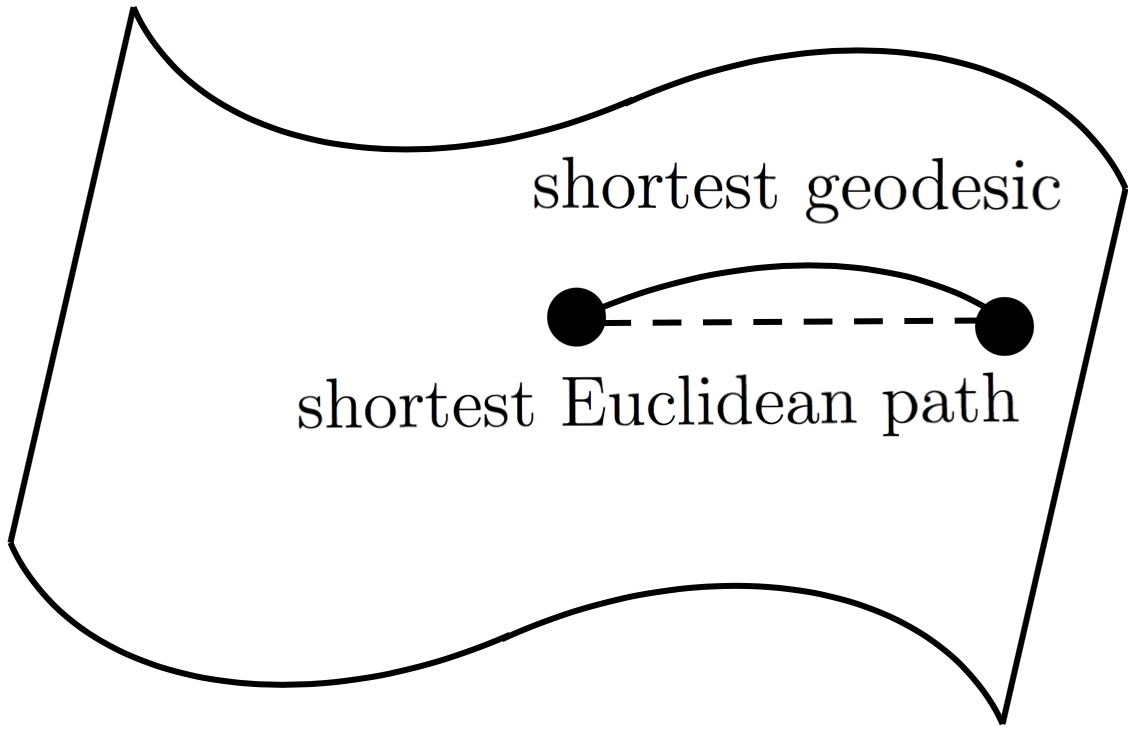
\includegraphics[scale=0.15]{chapter_1/files/geodesic.jpg}
    \caption{A manifold $\mathcal{M}$ embedded in some Euclidean
    space $\mathbb{R}^n$ may have a shortest geodesic that is
    not the same as the shortest Euclidean path.}
    \label{fig:geodesic}
\end{figure}
\begin{example}[Graph metric] The shortest path on graphs (for 
example a social network graph) forms a valid distance function. The
distance is just the smallest number of edges between two vertices.
\end{example}
\begin{remark}
A metric space isn't always a Euclidean space. So, we cannot always
perform Euclidean operations (ie. taking the mean) in an arbitrary
metric space.
\end{remark}

A metric gives a space a notion of distance or similarity. A natural
concept of a \emph{covering} helps us give a space a notion of size.

\begin{definition}[Cover]
Let $S \subset \mathcal{X}$, $\epsilon \geq 0$. A set $T \subset
\mathcal{X}$ is an $\epsilon$-cover of $S$ if:  $\forall s \in S$,
$\exists t \in T$ s.t. $\rho(s,t) \le \epsilon$.
\end{definition}

In other words, $T$ $\epsilon$-covers $S$ if $\sup_{s\in S} 
\rho(s,T)\leq \epsilon$.

\begin{exercise}
(i) Is $S$ a cover of $S$? (ii) Give the vertices $d$-dimensional
cube $\{-1,1\}^d$ the $\ell_\infty$ distance. What is a good 1-cover?
$\frac{1}{2}$-cover? $\frac{9}{10}$-cover?
\end{exercise}

\section{The \emph{k}-centers problem}
Consider the following optimization problem on an arbitrary metric
space:
\begin{enumerate}
\item \underline{Input}: a set of $n$ points $x_1,....x_n \in 
\mathcal{X}$ assuming $(X,\rho)$; a positive integer $k$ 
\item \underline{Output}: $T \subset \mathcal{X}$ s.t. $|T| = k$
\item \underline{Goal}: minimize the cost of $T$ where: $ cost(T)
:= \max_{i \in \{1...n\}} \rho(x_i,T) $
\end{enumerate}

One possible solution is an exhaustive search, which has exponential
time complexity. In fact, this problem is NP-hard, so we might look
instead for an approximate solution. The farthest first traversal
algorithm, which has polynomial complexity, does this.

\begin{algorithm}
\caption{Farthest First Traversal Algorithm (FFTA)}
\begin{algorithmic} 
\STATE Pick randomly $z\in \mathcal{X}$ and set $T = \{z\}$\;
\WHILE{$|T| < k$}
\STATE $z = \argmax_{x\in \mathcal{X}} \rho(x,T)$ \;
\STATE $T = T \cup \{z\}$\;
\ENDWHILE
\end{algorithmic}
\end{algorithm}

\begin{example}
To see that this is not an optimal solution to the k-center problem,
consider the following counterexample. Define the 2-center problem
($|T| = 2$) on the space $\mathcal{X} = \{0, \frac{1}{4}, \frac{1}{2},
\frac{3}{4}, 1\}$, with the usual metric $\rho$. The farthest fast
traversal algorithm might yield to  $\{0,1\}$ while the optimal
solution is $\{\frac{1}{4},\frac{3}{4}\}$.
\end{example}

\begin{theorem}
Let $T^*$ be the optimal solution of the k-center problem and
$\mathrm{cost}(T^*)$ be its optimal cost. Let T be a solution given
by FFTA. Then: 
\[cost(T^*) \le cost(T) \le 2 * cost(T^*)\]
Thus, FFTA is 2-optimal for the k-center problem. 
\end{theorem} 

\begin{proof}
Let $ cost(T) = r = \max_{s \in \mathcal{X}} \rho(s,T) $. There exists
$x_0 \in \mathcal{X}$ such that $x_0 = \argmax_{x \in\mathcal{X}}
\rho(x,T)$. We set $T' = T \cup \{x_0\} $, and observe that $\forall
t_i, t_j \in T', t_i \ne t_j : \rho(t_i,t_j) \ge r$, because if $x_0
\notin T$, then during any iteration of the farthest first traversal
algorithm, for the new center $t_i$ added to $T$ it must be true that
$\rho(t_i, T) \geq r$, otherwise $x_0$ would be already added to $T$.
We note that $|T'| = k+1$ and $ |T^*| = k$. Because there are $k$
elements in $T^*$ covering $k+1$ elements in $T'$, by the pigeonhole
principle, there exists some $t^* \in T^*$ that covers at least two
elements $t_1,t_2 \in T'$. As $\rho(t_1,t_2) \geq r$, by the triangle
inequality, at least one of $\rho(t_1,t^*)$ or $\rho(t_2,t^*)$ is at
least $\frac{r}{2}$. This implies $\mathrm{cost}(T^*)\geq\frac{r}{2}$.
\end{proof}

\begin{remark}
Obtaining an $(2 - \epsilon)$-approximation is NP-hard for general
metric spaces.
\end{remark}

\noindent\textbf{Some related open problems:} Hardness in Euclidean
spaces. Is k-center problem still hard in these spaces? Can we get
better than 2-optimality? Is this the better algorithm to solve the
problem? 

\section{The \emph{k}-means problem}
The $k$-means optimization problem is defined as:
\begin{enumerate}
\item \underline{Input}: A set of $n$ points $x_1,....x_n \in
\mathbb{R^d}$ and a positive integer $k<n$.
\item \underline{Output}: $T \subset  \mathbb{R^d}$ s.t. $|T|=k$. 
\item \underline{Goal}: minimize "cost" of $T$ where: $cost(T) 
:= \sum_{i = 1}^{n} \min_{\mu_j \in T} \norm{x_i-\mu_j}^2 $.
\end{enumerate}

As before, we can attempt and exhaustive search with exponential
time complexity. If we want some solution in polynomial time, we
must settle for an approximation, as $k$-means is also an NP-hard
optimization problem. One approximate solution is Lloyd's method
for $k$-means:

\begin{algorithm}
\caption{Lloyd k-means algorithm}
\begin{algorithmic} 
\STATE Pick randomly $x_1,...,x_k $ from $\mathcal{X}$ \;
\WHILE{stopping criteria not satisfied}
\STATE Assign points of the dataset to the closest center \;
\STATE Get the clusters $C_1, ..., C_k$\;
\STATE Compute the new centroïds $\mu_j = \frac{1}{|C_j|}
\sum_{x_i\in C_j} x_i$, $\forall j \in \{1,...,k\}$\;
\ENDWHILE
\end{algorithmic}
\end{algorithm}

\begin{remark}
As $k$-means is NP hard, Lloyd's method gives us an approximate
solution. However, we cannot give any approximation guarantees
on the solution, as the approximation may be arbitrarily bad.
\end{remark}

\begin{example} Consider the following setting and dataset
where $k=2$ and $d=1$:
\begin{figure}
    \centering
    \captionsetup{width=0.8\textwidth}
    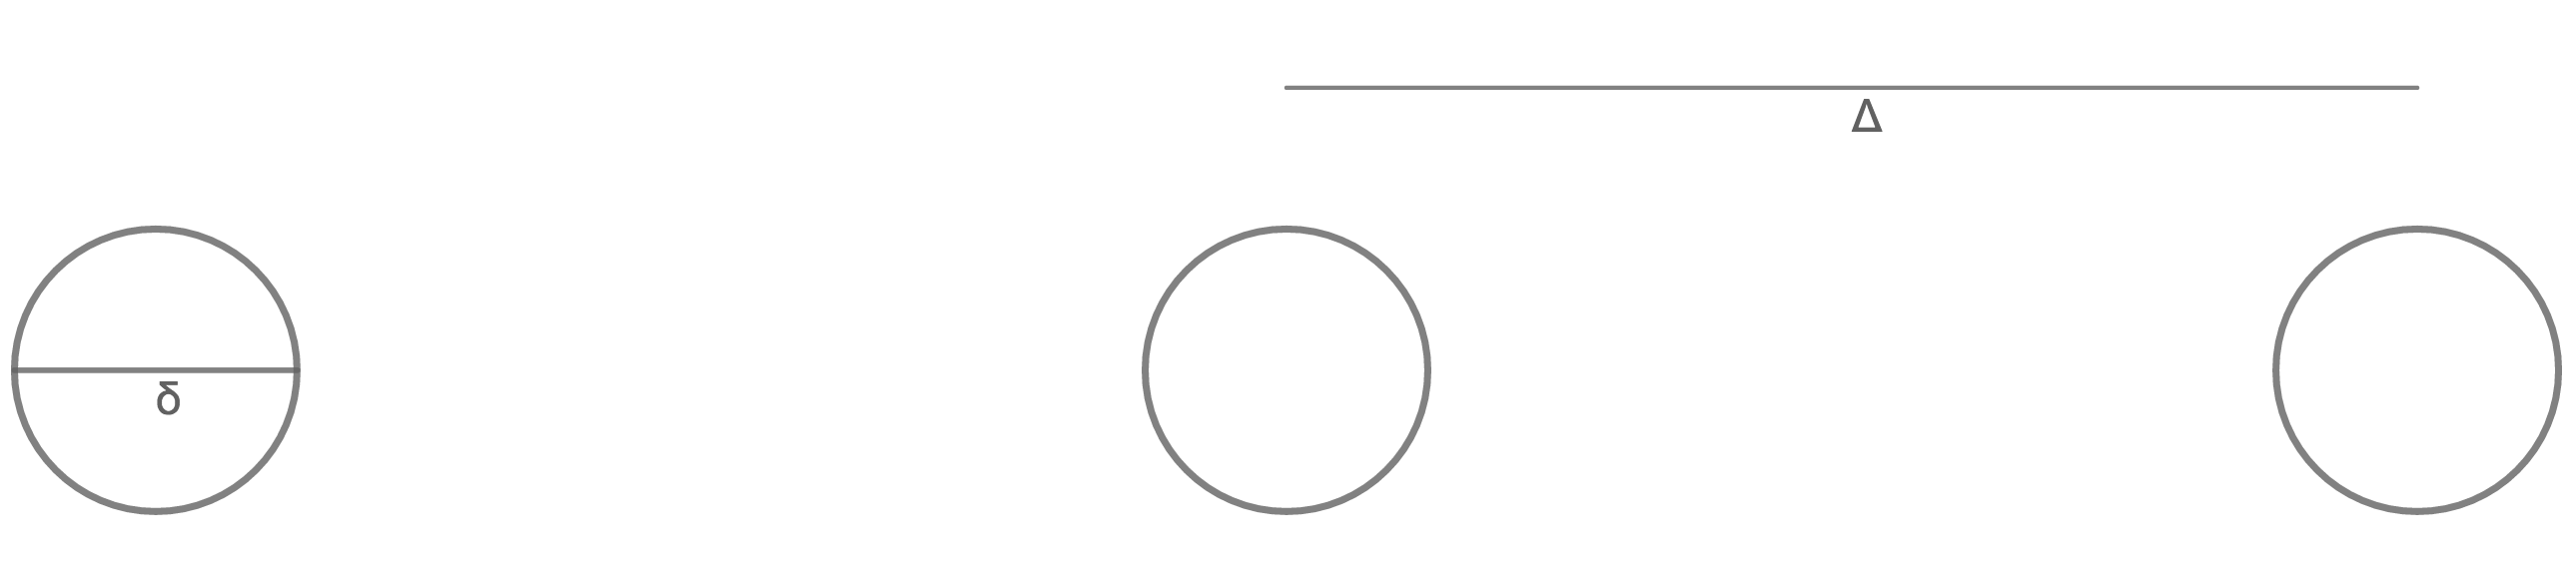
\includegraphics[scale=0.4]{chapter_1/files/kmeans.png}
    \caption{An example of datapoints and initial setting where
    Lloyd's algorithm fails to be optimal.}
    \label{fig:kmeans}
\end{figure}
The dashed lines point to the current cluster centers, with 0
for the blue cluster and 28 for the red cluster. On this
setting, Lloyd's algorithm makes no further improvement (it
terminates after one iteration), since the middle point at 16
is closer to the red cluster center 28 than to the blue cluster
center 0. And the total cost is $0^2+12^2+12^2=288$.

However, the optimal cluster center assignment should be 8 for
the blue cluster and 40 for the red cluster, which gives a cost
of $8^2+8^2+0^2=128$. Thus, Lloyd's algorithm does not give the
optimal solution.
\end{example}

\section{Further reading}
For a general reference to clustering algorithms, see \cite{har75}
or \cite{gon85}. On the hardness of $k$-means, see \cite{das2008}.
A local search approximation is given in \cite{kan2004}. The 
$k$-means++ algorithm is in \cite{art2007}.